\chapter{Concept}\label{ch:concept}
\section{System-model}\label{sec:model}
In this section, we define the system model that serves as the foundation for the concept of the generated task sets.
It is reduced to a description of the task model and the execution model without further defining a hardware model, since the generated model is designed to be a meta model with no constraints on hardware specifications, making it hardware independent.

\subsection{Task Model}\label{sec:task_model}
As a foundation for this generator, the following section defines the bounds and properties of tasks, jobs, and sets of tasks. This builds upon the basic concepts introduced in \cref{sec:tasks_and_jobs}, providing a more formal description with additional properties and information.

\subsubsection{Tasks}\label{sec:task}
Each task $\tau_i$ may be described by multiple points of time:
\begin{itemize}
    \item $a_i$: time of arrival
    \item $r_i$: release time
    \item $d_i$: deadline.
\end{itemize}
In this model, tasks are periodic with implicit deadlines, meaning that the arrival time $a_i$, release time $r_i$, and deadline $d_i$ can all be described by a single period value $T_i$. 
Specifically, the arrival time $a_i$ is the start of the period, the release time $r_i$ is the same as the arrival time, and the deadline $d_i$ is the end of the period. 
This simplifies the task model as follows:
\begin{itemize}
    \item $a_i = k \cdot T_i$
    \item $r_i = a_i$
    \item $d_i = (k + 1) \cdot T_i$
\end{itemize}
where $k$ is a non-negative integer representing the $k$-th instance of the task.
This restriction is applied for the same reason mentioned by \textcite{dar-tzenpengAssignmentSchedulingCommunicating1997}, as the allocation of aperiodic tasks can be considered ``a dynamic load sharing problem''\cite{dar-tzenpengAssignmentSchedulingCommunicating1997}. 
With aperiodic tasks, it is a challenge in itself to manage the additional tasks and react to them just in time.
Focusing on periodic tasks with implicit deadlines allows for a predictable schedule that is better to handle.
Adding aperiodic tasks may be an aspect to implement in the future, with a look onto the principle applied by \textcite{dar-tzenpengAssignmentSchedulingCommunicating1997}.

Given that the proposed generator leverages detailed knowledge about the execution times of task jobs, additional details are provided to describe it. 
Each task is assigned multiple execution times, representing the possible outcomes depending on the system's status when scheduled. This includes adding a list of possible execution times.
While $e_{i,k}$ defines the actual execution time of a job $\tau_{i,k}$\cite{buttazzoHardRealTimeComputing2024}, let's define $e_{{i,k}^poss}$ as a \textit{possible} runtime of the job.
This will be described in more detail in \cref{sec:job}.

\subsubsection{Task-set}\label{sec:taskset}
Two or more tasks would be considered a task set.
In this model, a task-set $\Gamma$ is simply represented as a set of all given $n$ tasks $\Gamma \coloneqq \{\tau_1, \tau_2, \ldots, \tau_n\}$.

To provide some interaction and influence between multiple tasks a chain $\Gamma^c$ is presented.
The model of a chain is widely described in research\cite{
beckerSynthesizingJoblevelDependencies2016,abdullahWorstcaseCauseeffectReaction2019,choiChainBasedFixedPriorityScheduling2020}.
A chain $\Gamma^c$ describes an \textit{ordered} list of tasks $\tau_1$ to $\tau_m$.
\begin{center}
    $\Gamma^c \coloneqq [\tau_s,\tau_{m_1},\tau_{m_2}, \ldots, \tau_e]$
\end{center}
\begin{itemize}
    \item $\tau_s$: the first task of the chain
    \item $\tau_{m_*}$: intermediate task of the chain
    \item $\tau_e$: the last task of the chain
\end{itemize}
Each element of that list is denoted with its index as $\Gamma^c[i]$ where $\Gamma^c[1]$ represents the first list element $\tau_s$\cite{choiChainBasedFixedPriorityScheduling2020}.
The elements in the list are ordered so the influence of the tasks is structured as $\tau_{m_x} \rightarrow \tau_{m_{x+1}}$.
A task $\tau_{m_{x+1}}$ is dependent on the outcome of $ \tau_{m_{x}}$.
The interaction between two tasks is done via shared memory on the premise the value is read at the start of a job and written at the end of a job\cite{choiChainBasedFixedPriorityScheduling2020}.
This corresponds to the model described in \cref{sec:let} of \ac{LET}.

Each task set generated by this scheduler is designed to be a harmonic task set, meaning that the periods of all tasks are multiples of each other\cite{liuSchedulingAlgorithmsMultiprogramming1973,kuoLoadAdjustmentAdaptive1991}.
As \textcite{liuSchedulingAlgorithmsMultiprogramming1973} state, it will allow the system to reach a utilization of up to $1$, whereas any non-harmonic set of tasks, when using a fixed-priority rate monotonic scheduling algorithm, will be bound in its (lower) utilization.

\subsubsection{Jobs}\label{sec:job}
A job $\tau_{i,k}$ represents a single instance of a task $\tau_i$ (see \cref{sec:tasks_and_jobs}) and is characterized by the following properties:
\begin{itemize}
    \item $k$: index of the job $\tau_{i,k}$ with $k \epsilon [0, \ldots, hyperperiod / \max(T_*)]$
    \item $r_{i,k}$: release time of job $\tau_{i,k}$
    \item $d_{i,k}$: deadline of job $\tau_{i,k}$
    \item $e_{i,k}$: computational time of job $\tau_{i,k}$
\end{itemize}

Due to being a harmonic task-set and its properties (see \cref{sec:scheduling}), the \textit{planning cycle}\cite{dar-tzenpengAssignmentSchedulingCommunicating1997} of $\Gamma$ is defined by the \textit{\ac{LCM}} of all tasks' periods $\{T_1, \ldots, T_n\}$, resulting in the period $T_{max}$ of the task with the highest period. 

As in \cref{sec:task} presented the possible execution times $e_{{i,k}^poss}$ describe possible execution times a job $\tau_{i,k}$ may be assigned.
In \cref{sec:concept_lower_execution_times} explains the execution times' generation in more detail.

Each task $\tau_i$ is characterized by its period $T_i$, its list of possible execution times $\{e_{{i,1}_poss}, e_{{i,2}_poss}, \ldots\}$, and the set of related jobs $\tau_i=\{\tau_{i_0}, \tau_{i_1}, \dots, \tau_{i_m}; m = \frac{P_{max}}{P_i} - 1\}$.

Each job $\tau_{i_j}$ is described by the release time $r_{i_m}$, the beginning of the next period $P_i+1$ is equal to the implicit deadline $d_i$, and the job's computational time $C_{i_m}$. The release time $r_{i_m}$ per job is set to be aligned with the period beginning with $0$.
\begin{center}
    $r_{i_m} = P_i \times m$ \\
    $d_{i_m} = P_i + r_{i_m}$
\end{center}
\todo{explain chains and their length}

\subsection{Execution Model}\label{sec:execution_model}
As already mentioned in \cref{sec:taskset} the employed scheduler will be a fixed-priority rate-monotonic scheduler (see \cref{sec:scheduling}).
The scheduler operates by assigning each task $\Tau_i$ a priority inversely proportional to its period $P_i$\ref{liuSchedulingAlgorithmsMultiprogramming1973}.
Tasks with shorter periods receive higher priorities and are scheduled more frequently.
Higher-priority tasks can preempt lower-priority tasks.
Suppose a higher-priority task becomes ready to execute while a lower-priority task is running. In that case, the scheduler will interrupt the lower-priority task and allocate the processor to the higher-priority task.
This is represented in the resulting schedule as jobs being divided into multiple segments $C_{i,k}^1$ to $C_{i,k}^j$ where $j$ is equal to the number of preemptions plus $1$.
The resulting schedule is a list of $C_{i,k}^j$ depicting the complete schedule.
Each $C_{i,k}^j$ has its own starting time $s_{i,k}^j$ and its finishing time $s_{i,k}^j$.

Making use of the \ac{RMS} in combination with the in \cref{sec:task_model} mentioned harmonic task-set, it is possible to reach utilizations up to $1$\cite{liuSchedulingAlgorithmsMultiprogramming1973}.

\textcite[p. 70f]{buttazzoHardRealTimeComputing2024} explains some assumptions to consider in the scheduling:
\begin{enumerate}
    \item[A1] The instances of a periodic task $\tau_i$ are regular
    \item[A2]. The instances of a periodic task $\tau_i$ are regularly activated at a constant rate. The interval $\Tau_i$ between two consecutive activations is the period of the task. 
    \item[A3]. All instances of a periodic task $\tau_i$ have the same worst-case execution time $C_i$.
    \item[A4]. All instances of a periodic task $\tau_i$ have the same relative deadline $d_i$, which is equal to the period .$\Tau_i$. 
    \item[A5]. All tasks in $\Tau$ are independent; that is, there are no precedence relations and no resource constraints.
    \item[A6]. No task can suspend itself, for example, on I/O operations. 
    \item[A7]. All tasks are released as soon as they arrive. 
    \item[A8]. All overheads in the kernel are assumed to be zero. 
\end{enumerate}
1
\todo{buttazzoHardRealTimeComputing2024 explains scheduling with some assumptions}

\cite{dar-tzenpengAssignmentSchedulingCommunicating1997}


\section{Workflow of Generation}\label{sec:concept}
The general workflow involves several key steps.

\cref{sec:generating_period_times} describes how the harmonic period times are picked.
\cref{sec:concept_task_chains} explains the idea of how it is decided what tasks will be influencing each other and how the dependency is depicted in the resulting model.
\cref{sec:period_tree, sec:concept_load_spread} explain the concept of representing the planning cycle with the task-sets periods as a tree graph.
\cref{sec:concept_lower_execution_times} \subsection{Variation of Execution Times}
\cref{sec:concept_job_chains} describes the variation of the task chains with final time values to be scheduled.
\cref{sec:concept_scheduler} paints the idea of how the tree graph may be used to create a schedule.

\subsection{Generating Period Times}\label{sec:generating_period_times}
For the purpose of keeping the generated task-set harmonic, the periods to which the tasks will be assigned are generated first.
The period being an abstract value in this scenario, the starting value in the generation is selected to be equal to $1$.
Every further period is selected by randomly choosing an integer value to multiply the current value with.
With the multiplication defining the number of jobs being generated, it may be favorable to keep this randomly chosen integer relatively small whilst being at minimum the value of $2$. 
This is done until a previously defined amount of values is generated, limiting the maximum length of the inter-task communication chains.

With the multiplication of the previous value a harmonic task-set is assured, since the \ac{LCM} is per definition the biggest generated period value.
In \cref{fig:chain_of_periods}, the maximum value is $24$, being a multiple of all lower periods.
Hence the planning cycle matches with the highest period of the task-set, in the given example the resulting time frame used to create the model is $[0,24[$.

\begin{figure}[ht]
    \begin{subfigure}[c]{0.45\textwidth}
        \resizebox{\textwidth}{!}{%
            \label{fig:chain_of_periods}
        % \usetikzlibrary{patterns} % Load patterns library
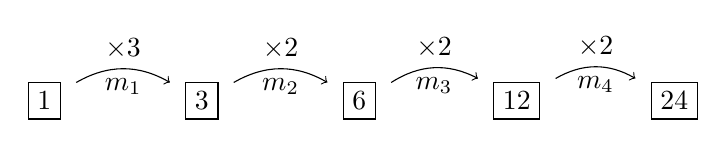
\begin{tikzpicture}
	% \node[draw, rectangle, outer sep=2mm] (n1) at (0,0) {1};
	% \node[draw, rectangle, outer sep=2mm] (n2) at (2,0) {3};
	% \node[draw, rectangle, outer sep=2mm] (n3) at (4,0) {6};
	% \node[outer sep=2mm] (n4) at (6,0) {\ldots};
	% \node[draw, rectangle, outer sep=2mm] (n5) at (8,0) {x};

	% \draw[->, bend left] (n1) tonode[midway,below] {$m_1$} node[midway,above] {$\times 3$} (n2);
	% \draw[->, bend left] (n2) tonode[midway,below] {$m_2$} node[midway,above] {$\times 2$} (n3);
	% \draw[->, bend left] (n3) tonode[midway,below] {$m_3$}  (n4);
	% \draw[->, bend left] (n4) tonode[midway,below] {$m_{n-1}$}  (n5);
	
	\node[draw, rectangle, outer sep=2mm] (n1) at (0,0) {1};
	\node[draw, rectangle, outer sep=2mm] (n2) at (2,0) {3};
	\node[draw, rectangle, outer sep=2mm] (n3) at (4,0) {6};
	\node[draw, rectangle, outer sep=2mm] (n4) at (6,0) {12};
	\node[draw, rectangle, outer sep=2mm] (n5) at (8,0) {24};

	\draw[->, bend left] (n1) to node[midway,below] {$m_1$} node[midway,above] {$\times 3$} (n2);
	\draw[->, bend left] (n2) to node[midway,below] {$m_2$} node[midway,above] {$\times 2$} (n3);
	\draw[->, bend left] (n3) to node[midway,below] {$m_3$} node[midway,above] {$\times 2$} (n4);
	\draw[->, bend left] (n4) to node[midway,below] {$m_4$} node[midway,above] {$\times 2$} (n5);
\end{tikzpicture}
 }
        \caption{Generation of a small example series of periods by multiplication}
    \end{subfigure}
    \hfill
    \begin{subfigure}[c]{0.45\textwidth}
        \resizebox{\textwidth}{!}{%
            \label{fig:chain_of_tasks}
            % \usetikzlibrary{patterns} % Load patterns library
\begin{tikzpicture}
	% \node[draw, rectangle, outer sep=2mm] (n1) at (0,0) {1};
	% \node[draw, rectangle, outer sep=2mm] (n2) at (2,0) {3};
	% \node[draw, rectangle, outer sep=2mm] (n3) at (4,0) {6};
	% \node[outer sep=2mm] (n4) at (6,0) {\ldots};
	% \node[draw, rectangle, outer sep=2mm] (n5) at (8,0) {x};

	% \draw[->, bend left] (n1) tonode[midway,below] {$m_1$} node[midway,above] {$\times 3$} (n2);
	% \draw[->, bend left] (n2) tonode[midway,below] {$m_2$} node[midway,above] {$\times 2$} (n3);
	% \draw[->, bend left] (n3) tonode[midway,below] {$m_3$}  (n4);
	% \draw[->, bend left] (n4) tonode[midway,below] {$m_{n-1}$}  (n5);
	
	\node[draw, rectangle, outer sep=2mm] (n1) at (0,0) {$P=1$};
	\node[draw, rectangle, outer sep=2mm] (n2) at (2,0) {$P=3$};
	\node[draw, rectangle, outer sep=2mm] (n3) at (4,0) {$P=6$};
	\node[draw, rectangle, outer sep=2mm] (n4) at (6,0) {$P=12$};
	\node[draw, rectangle, outer sep=2mm] (n5) at (8,0) {$P=24$};

	\node[draw, rectangle, outer sep=2mm] (n1) at (-1.5,-1) {chain 1};
	\node[draw, rectangle, outer sep=2mm] (n2) at (-1.5,-2) {chain 2};
	\node[draw, rectangle, outer sep=2mm] (n3) at (-1.5,-3) {chain 3};

	\draw[thick, fill=black!60, pattern=none] plot[] coordinates { (-0.5 + 0, -0.5)	(0.5 + 0, -0.5)	(0.5 + 0, -3.5)	(-0.5 + 0,-3.5)	} -- cycle;
	\draw[thick, fill=black!60, pattern=none] plot[] coordinates { (-0.5 + 2, -0.5)	(0.5 + 2, -0.5)	(0.5 + 2, -3.5)	(-0.5 + 2,-3.5)	} -- cycle;
	\draw[thick, fill=black!60, pattern=none] plot[] coordinates { (-0.5 + 4, -0.5)	(0.5 + 4, -0.5)	(0.5 + 4, -3.5)	(-0.5 + 4,-3.5)	} -- cycle;
	\draw[thick, fill=black!60, pattern=none] plot[] coordinates { (-0.5 + 6, -0.5)	(0.5 + 6, -0.5)	(0.5 + 6, -3.5)	(-0.5 + 6,-3.5)	} -- cycle;
	\draw[thick, fill=black!60, pattern=none] plot[] coordinates { (-0.5 + 8, -0.5)	(0.5 + 8, -0.5)	(0.5 + 8, -3.5)	(-0.5 + 8,-3.5)	} -- cycle;

	% chain 1
	\node[draw, rectangle, outer sep=1mm] (T1) at (0,-1) {$\Tau_1$};
	\node[draw, rectangle, outer sep=1mm] (T2) at (2,-1) {$\Tau_2$};
	\node[draw, rectangle, outer sep=1mm] (T3) at (4,-1) {$\Tau_3$};
	\node[draw, rectangle, outer sep=1mm] (T4) at (6,-1) {$\Tau_4$};
	\node[draw, rectangle, outer sep=1mm] (T5) at (8,-1) {$\Tau_5$};
	
	% chain 2
	\node[draw, rectangle, outer sep=1mm] (T6) at (0,-2) {$\Tau_6$};
	\node[draw, rectangle, outer sep=1mm] (T7) at (2,-2) {$\Tau_7$};
	% 												
	\node[draw, rectangle, outer sep=1mm] (T8) at (6,-2) {$\Tau_8$};
	% 											
	
	% chain 3
	\node[draw, rectangle, outer sep=1mm] (T9) at (0,-3) {$\Tau_9$};
	\node[draw, rectangle, outer sep=1mm] (T10) at (2,-3) {$\Tau_{10}$};
	\node[draw, rectangle, outer sep=1mm] (T11) at (4,-3) {$\Tau_{11}$};
	%
	%
  

\draw[->] (T1) to (T2);
\draw[->] (T2) to (T3);
\draw[->] (T3) to (T4);
\draw[->] (T4) to (T5);
\draw[->] (T6) to (T7);
\draw[->] (T7) to (T8);
\draw[->] (T9) to (T10);
\draw[->] (T10) to (T11);

% \draw[->, bend left] (n1) to node[midway,below] {$m_1$} node[midway,above] {$\times 3$} (n2);

		

\end{tikzpicture}
 }
        \caption{Task-set $\Tau=\{\Tau_{1}, \ldots, \Tau_{11}\}$ parted into three subsets, each a representation of a chain of inter-task communication}
    \end{subfigure}
    \begin{subfigure}[c]{0.450\textwidth}
        \resizebox{\textwidth}{!}{%
            \label{fig:graph_of_periods}
            % \usetikzlibrary{patterns} % Load patterns library
\begin{tikzpicture}
	\node[draw, circle, inner sep=1mm] (L1-00) at (23 , 8) {$P2_-00$};

	\node[draw, circle, inner sep=1mm] (L2-00) at (11 , 6) {$P1_-00$};
	\node[draw, circle, inner sep=1mm] (L2-01) at (35 , 6) {$P1_-01$};

	\node[draw, circle, inner sep=1mm] (L3-00) at ( 5 , 4) {$P6_00$};
	\node[draw, circle, inner sep=1mm] (L3-01) at (17 , 4) {$P6_01$};
	\node[draw, circle, inner sep=1mm] (L3-02) at (29 , 4) {$P6_02$};
	\node[draw, circle, inner sep=1mm] (L3-03) at (41 , 4) {$P6_03$};

	\node[draw, circle, inner sep=1mm] (L4-00) at ( 2 , 2) {$P3_00$};
	\node[draw, circle, inner sep=1mm] (L4-01) at ( 8 , 2) {$P3_01$};
	\node[draw, circle, inner sep=1mm] (L4-02) at (14 , 2) {$P3_02$};
	\node[draw, circle, inner sep=1mm] (L4-03) at (20 , 2) {$P3_03$};
	\node[draw, circle, inner sep=1mm] (L4-04) at (26 , 2) {$P3_04$};
	\node[draw, circle, inner sep=1mm] (L4-05) at (32 , 2) {$P3_05$};
	\node[draw, circle, inner sep=1mm] (L4-06) at (38 , 2) {$P3_06$};
	\node[draw, circle, inner sep=1mm] (L4-07) at (44 , 2) {$P3_07$};

	\node[draw, circle, inner sep=1mm] (L5-00) at ( 0 , 0) {$P1_00$};
	\node[draw, circle, inner sep=1mm] (L5-01) at ( 2 , 0) {$P1_01$};
	\node[draw, circle, inner sep=1mm] (L5-02) at ( 4 , 0) {$P1_02$};
	\node[draw, circle, inner sep=1mm] (L5-03) at ( 6 , 0) {$P1_03$};
	\node[draw, circle, inner sep=1mm] (L5-04) at ( 8 , 0) {$P1_04$};
	\node[draw, circle, inner sep=1mm] (L5-05) at (10 , 0) {$P1_05$};
	\node[draw, circle, inner sep=1mm] (L5-06) at (12 , 0) {$P1_06$};
	\node[draw, circle, inner sep=1mm] (L5-07) at (14 , 0) {$P1_07$};
	\node[draw, circle, inner sep=1mm] (L5-08) at (16 , 0) {$P1_08$};
	\node[draw, circle, inner sep=1mm] (L5-09) at (18 , 0) {$P1_09$};
	\node[draw, circle, inner sep=1mm] (L5-10) at (20 , 0) {$P1_10$};
	\node[draw, circle, inner sep=1mm] (L5-11) at (22 , 0) {$P1_11$};
	\node[draw, circle, inner sep=1mm] (L5-12) at (24 , 0) {$P1_12$};
	\node[draw, circle, inner sep=1mm] (L5-13) at (26 , 0) {$P1_13$};
	\node[draw, circle, inner sep=1mm] (L5-14) at (28 , 0) {$P1_14$};
	\node[draw, circle, inner sep=1mm] (L5-15) at (30 , 0) {$P1_15$};
	\node[draw, circle, inner sep=1mm] (L5-16) at (32 , 0) {$P1_16$};
	\node[draw, circle, inner sep=1mm] (L5-17) at (34 , 0) {$P1_17$};
	\node[draw, circle, inner sep=1mm] (L5-18) at (36 , 0) {$P1_18$};
	\node[draw, circle, inner sep=1mm] (L5-19) at (38 , 0) {$P1_19$};
	\node[draw, circle, inner sep=1mm] (L5-20) at (40 , 0) {$P1_20$};
	\node[draw, circle, inner sep=1mm] (L5-21) at (42 , 0) {$P1_21$};
	\node[draw, circle, inner sep=1mm] (L5-22) at (44 , 0) {$P1_22$};
	\node[draw, circle, inner sep=1mm] (L5-23) at (46 , 0) {$P1_23$};

	\draw[->] (L1-00) to (L2-00);
	\draw[->] (L1-00) to (L2-01);

	\draw[->] (L2-00) to (L3-00);
	\draw[->] (L2-00) to (L3-01);
	\draw[->] (L2-01) to (L3-02);
	\draw[->] (L2-01) to (L3-03);

	\draw[->] (L3-00) to (L4-00);
	\draw[->] (L3-00) to (L4-01);
	\draw[->] (L3-01) to (L4-02);
	\draw[->] (L3-01) to (L4-03);
	\draw[->] (L3-02) to (L4-04);
	\draw[->] (L3-02) to (L4-05);
	\draw[->] (L3-03) to (L4-06);
	\draw[->] (L3-03) to (L4-07);

	\draw[->] (L4-00) to (L5-00);
	\draw[->] (L4-00) to (L5-01);
	\draw[->] (L4-00) to (L5-02);
	\draw[->] (L4-01) to (L5-03);
	\draw[->] (L4-01) to (L5-04);
	\draw[->] (L4-01) to (L5-05);
	\draw[->] (L4-02) to (L5-06);
	\draw[->] (L4-02) to (L5-07);
	\draw[->] (L4-02) to (L5-08);
	\draw[->] (L4-03) to (L5-09);
	\draw[->] (L4-03) to (L5-10);
	\draw[->] (L4-03) to (L5-11);
	\draw[->] (L4-04) to (L5-12);
	\draw[->] (L4-04) to (L5-13);
	\draw[->] (L4-04) to (L5-14);
	\draw[->] (L4-05) to (L5-15);
	\draw[->] (L4-05) to (L5-16);
	\draw[->] (L4-05) to (L5-17);
	\draw[->] (L4-06) to (L5-18);
	\draw[->] (L4-06) to (L5-19);
	\draw[->] (L4-06) to (L5-20);
	\draw[->] (L4-07) to (L5-21);
	\draw[->] (L4-07) to (L5-22);
	\draw[->] (L4-07) to (L5-23);

	\draw[line width=2mm, loosely dotted, pattern=none] plot[] coordinates { (-1, -1) (11, -1) (11, 5) (-1, 5) } -- cycle;
\end{tikzpicture}
 }
        \caption{A graph depicting the generated periods. Highlighted with a dotted box: subtree with $P6_0$ as root (see \cref{fid:graph_of_tasks}).}
    \end{subfigure}
    \hfill
    \begin{subfigure}[c]{0.45\textwidth}
        \resizebox{\textwidth}{!}{%
            \label{fig:graph_of_tasks}
            % \usetikzlibrary{patterns} % Load patterns library
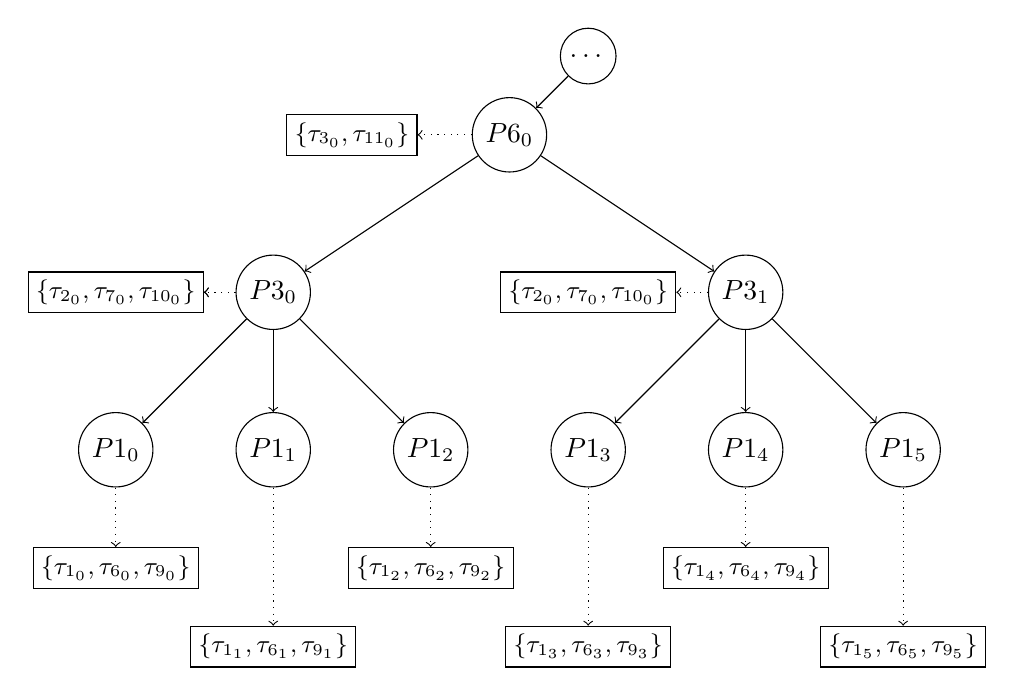
\begin{tikzpicture}
	\node[draw, circle, inner sep=1mm] (L2-00) at ( 6, 5) {\ldots};

	\node[draw, circle, inner sep=1mm] (L3-00) at ( 5 , 4) {$P6_0$};

	\node[draw, circle, inner sep=1mm] (L4-00) at ( 2 , 2) {$P3_0$};
	\node[draw, circle, inner sep=1mm] (L4-01) at ( 8 , 2) {$P3_1$};

	\node[draw, circle, inner sep=1mm] (L5-00) at ( 0 , 0) {$P1_0$};
	\node[draw, circle, inner sep=1mm] (L5-01) at ( 2 , 0) {$P1_1$};
	\node[draw, circle, inner sep=1mm] (L5-02) at ( 4 , 0) {$P1_2$};
	\node[draw, circle, inner sep=1mm] (L5-03) at ( 6 , 0) {$P1_3$};
	\node[draw, circle, inner sep=1mm] (L5-04) at ( 8 , 0) {$P1_4$};
	\node[draw, circle, inner sep=1mm] (L5-05) at (10 , 0) {$P1_5$};

	\node[draw, rectangle, inner sep=1mm, align=center] (L3-T00) at ( 3 , 4) {\small $\{\tau_{3_0},\tau_{11_0}\}$};

	\node[draw, rectangle, inner sep=1mm, align=center] (L4-T00) at ( 0 , 2) {\small $\{\tau_{2_0},\tau_{7_0},\tau_{10_0}\}$};
	\node[draw, rectangle, inner sep=1mm, align=center] (L4-T01) at ( 6 , 2) {\small $\{\tau_{2_0},\tau_{7_0},\tau_{10_0}\}$};

	\node[draw, rectangle, inner sep=1mm, align=center] (L5-T00) at ( 0 , -1.5) {\small $\{\tau_{1_0},\tau_{6_0},\tau_{9_0}\}$};
	\node[draw, rectangle, inner sep=1mm, align=center] (L5-T01) at ( 2 , -2.5) {\small $\{\tau_{1_1},\tau_{6_1},\tau_{9_1}\}$};
	\node[draw, rectangle, inner sep=1mm, align=center] (L5-T02) at ( 4 , -1.5) {\small $\{\tau_{1_2},\tau_{6_2},\tau_{9_2}\}$};
	\node[draw, rectangle, inner sep=1mm, align=center] (L5-T03) at ( 6 , -2.5) {\small $\{\tau_{1_3},\tau_{6_3},\tau_{9_3}\}$};
	\node[draw, rectangle, inner sep=1mm, align=center] (L5-T04) at ( 8 , -1.5) {\small $\{\tau_{1_4},\tau_{6_4},\tau_{9_4}\}$};
	\node[draw, rectangle, inner sep=1mm, align=center] (L5-T05) at (10 , -2.5) {\small $\{\tau_{1_5},\tau_{6_5},\tau_{9_5}\}$};

	\draw[->] (L2-00) to (L3-00);

	\draw[->] (L3-00) to (L4-00);
	\draw[->] (L3-00) to (L4-01);

	\draw[->] (L4-00) to (L5-00);
	\draw[->] (L4-00) to (L5-01);
	\draw[->] (L4-00) to (L5-02);
	\draw[->] (L4-01) to (L5-03);
	\draw[->] (L4-01) to (L5-04);
	\draw[->] (L4-01) to (L5-05);

	\draw[->,dotted] (L3-00) to (L3-T00);
	\draw[->,dotted] (L4-00) to (L4-T00);
	\draw[->,dotted] (L4-00) to (L4-T00);
	\draw[->,dotted] (L4-01) to (L4-T01);
	\draw[->,dotted] (L5-00) to (L5-T00);
	\draw[->,dotted] (L5-01) to (L5-T01);
	\draw[->,dotted] (L5-02) to (L5-T02);
	\draw[->,dotted] (L5-03) to (L5-T03);
	\draw[->,dotted] (L5-04) to (L5-T04);
	\draw[->,dotted] (L5-05) to (L5-T05);

\end{tikzpicture}
 }
        \caption{Subgraph of \cref{fig:graph_of_periods} showing the jobs associated to each representation of period iteration}
    \end{subfigure}
    \caption{Generation of periods and task-set with tasks with given period}\label{fig:graph}
\end{figure}

\subsection{Generating Task Chains}\label{sec:concept_task_chains}
Multiple tasks will be iteratively added and assigned to the already generated periods to generate the task set.
By iterating about given period values a natural order of the tasks' periods is assured.
With choosing the \ac{RMS} as scheduling method it is an descending order of priority, since the higher periods will result in lower priorities.
Knowing this the tasks can be connected with its successor (if one does exist) to limit the inter-task communication to be directed from higher priorities to lower priorities.

Without \todo{!} 
By doing so, the sender is assured to run earlier with respect to the receiver if no locking or priority inversion is apparent. \todo{priority inversion and resource locking in model}
By skipping a period while generating the tasks, the chains are built to vary the length and distribution of their associated tasks.
The skip may be done at random.

\subsection{Period-tree}\label{sec:period_tree}
Using a harmonic task-set allows it to fan out the given list of periods as seen in \cref{fig:chain_of_periods} into a tree structure as seen in \cref{fig:graph_of_periods}.
Due to the periods being multiples of each other, the used multiple is the key to perfectly mapping the periods onto the same span of time.
Beginning with the smallest period, i.e., $1$, whilst ignoring periods greater than that for now, it perfectly represents the needed planning cycle $1$.
This is represented by node $P1_0$ in \cref{fig:graph_of_periods}.
If the next biggest period $3$ gets added into the picture, the planning cycle increases to $3$, resulting in three repetitions of the previous period to match the newer and bigger cycle, represented by $P3_0$ and $P1_0$ to $P1_2$ in \cref{fig:graph_of_periods}.
Repeating this for the remaining periods, the complete tree built so far will be multiplied and added.
The benefits of this design will be explained in more detail in \cref{sec:concept_scheduler}.

\subsection{Assigning Computational Time}\label{sec:concept_load_spread}
At this stage, the generated tasks have no computational time assigned.
The model is planned to satisfy a given utilization.
Taking that utilization, each period may be assigned a combined execution time to represent the sum of associated tasks.

The planning cycle's time frame, multiplied by the predefined utilization, determines the total amount of execution time that can be distributed across the tasks.
This means that for each layer of period nodes in the tree structure, the sum of the execution times of all tasks must not exceed the product of the planning cycle's time frame and the predefined utilization.

For example, if the planning cycle's time frame is $24$ units and the targeted utilization is $0.75$, the total execution time available for all tasks in that planning cycle is \(24 \times 0.75 = 18\) units.
This $18$ units of execution time must be spread across all tasks in the tree, ensuring that the sum of the execution times of tasks associated with each period node does not exceed this limit.

The total execution time for each period layer is then distributed among the tasks assigned to that period. This is done by randomly assigning execution times to each task such that the sum of the execution times equals the total execution time for the period layer.

\todo{rewrite}
For example, if a period layer of $P1$ has a total execution time of $12$ units and there are three tasks $T_1$, $T_3$ and $T_9$ assigned to that period, the execution times could be randomly assigned as $CP_{1_1} = 3$, $CP_{3_1} = 5$, and $CP_{9_1} = 5$, ensuring that the sum is \( CP_{1_1} + CP_{3_1} + CP_{9_1} = 6 \) units.

By randomly distributing the execution times in this manner, the system ensures that the overall utilization remains within the desired bounds, maintaining the schedulability and efficiency of the task set.

\subsection{Variation of Execution Times}\label{sec:concept_lower_execution_times}
For the system to not only represent all tasks' \ac{WCET}, a variation of execution times per task needs to be created.
Since the generated tasks with full load still have schedulability, the execution time of the tasks may be reduced without compromising the schedulability.
For that reason, the execution time of each task is multiplied by a random value between zero and one until a sufficient number of different values are generated.
Keeping the increasing complexity in mind, the system is designed to use a discrete distribution instead of continuous value functions to keep the possible permutations at considerable amounts.

\subsection{Generating Job Chains}\label{sec:concept_job_chains}
As \cref{sec:concept_task_chains} describes chains of tasks, there is the need to specify these to accommodate for the variations described in \cref{sec:concept_lower_execution_times}.
Whilst the previously created chains of tasks may describe a general dependency, it is now necessary to use the variations to calculate the actual chains being used in the schedule, as described in \cref{sec:concept_scheduler} later on.
For now, the creation is not bound to any restrictions and will end in a permutation of the created variations.

With multiple possible execution times per task, these variants need to be conditioned to ensure deterministic behavior.
This can be achieved by defining conditions that link the execution times of tasks within a chain, ensuring that the execution time of one task influences the execution time of subsequent tasks in the chain, as described in \cref{sec:concept_task_chains}.
The conditions are supposed to mimic the data flow between two tasks and the influence between these two.
The most simple attempt to combine the different variants of the two tasks together would be by pseudo-randomly assigning a follow-up variant of the second task to each of the first task's variants.
The biggest shortcoming with this idea would be the easy predictability of a chain since the first task would determine the execution times of the following tasks by transitivity.
To hide the effects, another independent input may be inserted into the condition, representing the environment's influence on the program.

% Having two array like structures for each tasks variants the independent input may be used as a shift to look up the condition to use.
% This could be as simple as using modulo calculations or any other hash function.

\begin{figure}[ht]
    % \begin{subfigure}[c]{0.45\textwidth}
        \resizebox{\textwidth}{!}{%
            \label{fig:conditions_a}
            \input{./tikz/conditions_a.tex}
 }
    %   \caption{Unshifted}
    % \end{subfigure}
    % \hfill
    % \begin{subfigure}[c]{0.45\textwidth}
    %   \resizebox{\textwidth}{!}{%
    %       \label{fig:conditions_b}
    %       % \usetikzlibrary{patterns} % Load patterns library
\begin{tikzpicture}	
	\node (A0) [draw, minimum width=1cm, minimum height=1cm, label={[font=\tiny, anchor=north west]north west:0}] {10};
	\node (A1) [draw, minimum width=1cm, minimum height=1cm, right=0cm of A0, label={[font=\tiny, anchor=north west]north west:1}] {25};
	\node (A2) [draw, minimum width=1cm, minimum height=1cm, right=0cm of A1, label={[font=\tiny, anchor=north west]north west:2}] {33};
	\node (A3) [draw, minimum width=1cm, minimum height=1cm, right=0cm of A2, label={[font=\tiny, anchor=north west]north west:3}] {79};
	\node (A4) [draw, minimum width=1cm, minimum height=1cm, right=0cm of A3, label={[font=\tiny, anchor=north west]north west:4}] {110};

	\node (B0) [draw, minimum width=1cm, minimum height=1cm, below=2cm of A0, label={[font=\tiny, anchor=north west]north west:0}] {7};
	\node (B1) [draw, minimum width=1cm, minimum height=1cm, right=0cm of B0, label={[font=\tiny, anchor=north west]north west:1}] {12};
	\node (B2) [draw, minimum width=1cm, minimum height=1cm, right=0cm of B1, label={[font=\tiny, anchor=north west]north west:2}] {21};
	\node (B3) [draw, minimum width=1cm, minimum height=1cm, right=0cm of B2, label={[font=\tiny, anchor=north west]north west:3}] {46};
	\node (B4) [draw, minimum width=1cm, minimum height=1cm, right=0cm of B3, label={[font=\tiny, anchor=north west]north west:4}] {70};

	\node (C0) [draw, minimum width=1cm, minimum height=1cm, below=2cm of B0, label={[font=\tiny, anchor=north west]north west:0}] {18};
	\node (C1) [draw, minimum width=1cm, minimum height=1cm, right=0cm of C0, label={[font=\tiny, anchor=north west]north west:1}] {30};
	\node (C2) [draw, minimum width=1cm, minimum height=1cm, right=0cm of C1, label={[font=\tiny, anchor=north west]north west:2}] {35};
	\node (C3) [draw, minimum width=1cm, minimum height=1cm, right=0cm of C2, label={[font=\tiny, anchor=north west]north west:3}] {42};
	\node (C4) [draw, minimum width=1cm, minimum height=1cm, right=0cm of C3, label={[font=\tiny, anchor=north west]north west:4}] {75};
 
	\node (TA) [minimum width=1cm, minimum height=0.5cm, left=0cm of A0] {$CP_i$ of $T_0$};
	\node (TB) [minimum width=1cm, minimum height=0.5cm, left=0cm of B0] {$CP_i$ of $T_1$};
	\node (TC) [minimum width=1cm, minimum height=0.5cm, left=0cm of C0] {$CP_i$ of $T_2$};
  
	\draw[->] (A0.south) -- (B1.north);
	\draw[->] (A1.south) -- (B3.north);
	\draw[->] (A2.south) -- (B2.north);
	\draw[->] (A3.south) -- (B0.north);
	\draw[->] (A4.south) -- (B4.north);
	
	\draw[->] (B0.south) -- (C1.north);
	\draw[->] (B1.south) -- (C0.north);
	\draw[->] (B2.south) -- (C3.north);
	\draw[->] (B3.south) -- (C4.north);
	\draw[->] (B4.south) -- (C2.north);
    
	\draw[red, thick] ($(A0.south west)+(-0.2,0.2)$) rectangle ($(B4.north east)+(0.2,-0.2)$);
	\node (redBoxText) [minimum width=1cm, minimum height=0.5cm] at (-2,-1.5) {Added shift: $3$};
	\draw[red, thick] ($(B0.south west)+(-0.2,0.2)$) rectangle ($(C4.north east)+(0.2,-0.2)$);
	\node (redBoxText2) [minimum width=1cm, minimum height=0.5cm] at (-2,-4.5) {Added shift: $2$};
	
\end{tikzpicture}
    %   }
    %   \caption{Shifted}
    % \end{subfigure}
    \caption{Generation of periods and task-set with tasks with given period}
\end{figure}

For example, consider a chain of tasks \( \tau_1 \{ CP: \{10,25,33,79,110\}\}, \tau_2 \{ CP: \{7,12,21,46,70\}\}, \tau_3 \{CP: \{18,30,35,42,75\} \).
We can define conditions such that the execution time of \( \tau_1 \) affects the execution time of \( \tau_2 \), and the execution time of \( \tau_2 \) affects the execution time of \( \tau_3 \). 
For instance, as displayed in \cref{fig:conditions_a}, the chain has multiple routes to traverse about the possible execution times.
For example, the first entry in the list of the tasks execution times would lead to index 3 in the second tasks list and finally get to index 2 in the third tasks list resulting in a specific chain \( \tau_1: 10 \rightarrow \tau_2: 46 \rightarrow \tau_3: 35 \).

By defining such conditions, we ensure that the execution times are linked and the overall behavior of the system remains predictable and deterministic. 
This approach helps maintain the schedulability and efficiency of the task set while accommodating variations in execution times.

\subsection{Building a Scheduler and Performing Schedulability Test}\label{sec:concept_scheduler}
The schedule can be generated by performing a depth-first traversal of the previously described tree structure.
The hightest prioritized tasks are added as leaves into thre tree and are processed first during the traversal.
As the traversal continues, tasks in higher layers with lower priorities are processed until the root is reached.
Starting with an empty schedule for the given planning cycle, the execution times of the highest prioritized tasks can simply be added.
If one layer is added to the schedule, the next layer with the next higher priority is added to the remaining idle time slots.
Since the time and utilization are previously calculated it is ensured the task set is schedulable.

\subsection{Using the chains}\label{sec:chains}
\todo{!!}
\todo{image of longest chains added}